% Created 2015-03-12 Thu 15:32
\documentclass[11pt]{article}
\usepackage[latin1]{inputenc}
\usepackage[T1]{fontenc}
\usepackage{fixltx2e}
\usepackage{graphicx}
\usepackage{longtable}
\usepackage{float}
\usepackage{wrapfig}
\usepackage{rotating}
\usepackage[normalem]{ulem}
\usepackage{amsmath}
\usepackage{textcomp}
\usepackage{marvosym}
\usepackage{wasysym}
\usepackage{amssymb}
\usepackage{hyperref}
\tolerance=1000
\usepackage[parfill]{parskip}
\usepackage{mathtools}
\usepackage[utf8]{inputenc}
\usepackage[swedish, english]{babel}
\usepackage[T1]{fontenc}
\usepackage{moreverb,fancyheadings,graphicx, amssymb}
\usepackage{fixltx2e}
\usepackage{longtable}
\usepackage{float}
\usepackage{wrapfig}
\usepackage{soul}
\usepackage{textcomp}
\usepackage{marvosym}
\usepackage{wasysym}
\usepackage{latexsym}
\usepackage{hyperref}
\author{Anton Erholt \& Christopher M�rtensson \\ <aerholt@kth.se> <cmarte@kth.se>}
\date{\today}
\title{Parallelized particle simulation}
\hypersetup{
  pdfkeywords={},
  pdfsubject={A project in the course ID1217 at KTH},
  pdfcreator={Emacs 24.4.1 (Org mode 8.2.10)}}
\begin{document}

\maketitle
\newpage
\begin{abstract}

This report serves to describe a programming project in the course
ID1217, Concurrent programming. The project was to implement an
algorithm for a parallel particle simulation which ran in time close to $O(T/p)$,
where $T$ is the running time of the algorithm running on $p$ processors.

\end{abstract}
\newpage

\section*{Introduction}
\label{sec-1}

This programming project is about finding an improved algorithm for
solving a particle simulation problem and implementing
it. Furthermore, the project consists of improving said implementation
by parallelizing it to several processors.

The particle simulation is made by a per-particle basis, applying the
force of its neighboring particles and recalculating the particle
position and velocity.

\section*{The algorithm}
\label{sec-2}

The algorithm we have chosen to implement is probably best known as
binning. We divide the field of particles into several 'bins' (like a
grid) which we then use to filter out which particles we should take
into account when calculating forces. Using a shared memory layout
with this type of design requires little to no changes for an actual
implementation. With a distributed memory layout, the design requires
a few additions.

The algorithm described in pseudo-code is:

\begin{verbatim}
P = set(Particle)
N = P.size()

def simulate_step():
    for particle in P:
        # Parallelize here
        neighbors = find_neighbors(particle)
        for n in neighbors:
            particle.applyForceOf(n)
        # Synchronize here
    return P
\end{verbatim}

Where the size of neighbors is significantly smaller than N and
therefore makes the binning algorithm's running time $\in O(N)$.

$$ neighbors.size() << N $$

The calculation part which we parallelize is obviously the force calculation for
every particle. This project limits itself not to discuss whether or
not one would gain anything from also parallelizing over several time
steps.

\section*{Implementation details}
\label{sec-3}

\subsection*{Shared memory layout}
\label{sec-3-1}

\subsubsection*{Serial}
\label{sec-3-1-1}
The serial solution uses no type of parallelization and runs the
binning algorithm as expected, in $O(n)$ time (where $n$ is the number
of particles).

\subsubsection*{OpenMP}
\label{sec-3-1-2}
The OpenMP version implements a parallel version of the binning
algorithm. It uses the \verb~#pragma omp parallel for~ directive for
parallelization and synchronization. The directive \verb~#pragma omp critical~ is used to ensure the critical region of the algorithm is
executed atomically.

\subsubsection*{Pthreads}
\label{sec-3-1-3}
The pthreads implementation uses more low level synchronization
primitives, namely a barrier for synchronization and a mutex for
locking. The particle array is split into as many chunks as we have
threads, and each thread gets to work on its own chunk.

\subsection*{Distributed memory layout}
\label{sec-3-2}

Using a distributed memory layout forces an addition in the algorithm
design. We partition the grid of particles into rows and make each row
an object of parallelization. Every row 'talks' to its neighbours on
top and below. This allows the row to send and receive the particles
closest to the edges for a more accurate description of the forces.


\subsubsection*{MPI}
\label{sec-3-2-1}
We estimate the contention of our implementation to be quite high, but
still being able to beat the non-linear implementation given.

\section*{Calculations and results}
\label{sec-4}

\subsection*{Linearity}
\label{sec-4-1}
By plotting the size of the input $n$ and the running time
$t_serial$ we conclude the linearity of our algorithm.

See Appendix for output of the actual runs.

\begin{center}
\begin{tabular}{rrrr}
n & t$_{\text{serial}}$ & log$_{\text{2}}$(t$_{\text{serial}}$) & log$_{\text{2}}$(n)\\
\hline
5000 & 2.530250 & 0.84499156 & 12.28771238\\
10000 & 5.798080 & 1.599769861 & 13.28771238\\
20000 & 9.404700 & 2.040036861 & 14.28771238\\
40000 & 23.231000 & 2.863146195 & 15.28771238\\
80000 & 54.164900 & 3.633705119 & 16.28771238\\
160000 & 110.290000 & 4.280958177 & 17.28771238\\
\end{tabular}
\end{center}

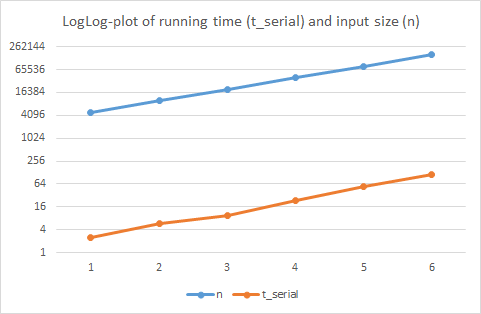
\includegraphics[width=.9\linewidth]{./loglog-serial.png}

\subsection*{Comparison of running times}
\label{sec-4-2}
\begin{center}
\begin{tabular}{lrrrr}
 & T & p=1 & p=2 & p=4\\
\hline
Serial & 1.0 & 1.0 & 1.0 & 1.0\\
OpenMP &  &  &  & \\
Pthreads &  &  &  & \\
MPI &  &  &  & \\
\end{tabular}
\end{center}


\section*{Discussion and thoughts}
\label{sec-5}

\textbf{TODO}


Speedup plots that show how closely your parallel codes approach the
idealized p-times speedup and a discussion on whether it is possible
to do better.

Where does the time go? Consider breaking down the runtime into
computation time, synchronization time and/or communication time. How
do they scale with p?

A discussion on using pthreads, OpenMP and MPI.

OpenMP = YES, GOD YES!
pthreads = Meh,
MPI = ARE YOU JOKING!?!?EIFJIDSOAJFaz


\section*{Plots and figures}
\label{sec-6}

\section*{Appendix}
\label{sec-7}

\subsection*{Serial (linearity)}
\label{sec-7-1}

\textbf{NOTE:} Some runs are omitted below. This is just an excerpt from were
the calculation numbers were taken.

\begin{verbatim}
[aerholt@localhost particles-pps14]$ ./linearserial -n 5000
size: 7.071068
integer size: 317
Scale: 44.830570
n = 5000, simulation time = 1.94145 seconds
[aerholt@localhost particles-pps14]$ ./linearserial -n 5000
size: 7.071068
integer size: 317
Scale: 44.830570
n = 5000, simulation time = 2.10103 seconds
[aerholt@localhost particles-pps14]$ ./linearserial -n 5000
size: 7.071068
integer size: 317
Scale: 44.830570
n = 5000, simulation time = 2.53025 seconds
[aerholt@localhost particles-pps14]$ ./linearserial -n 5000
size: 7.071068
integer size: 317
Scale: 44.830570
n = 5000, simulation time = 2.58599 seconds
[aerholt@localhost particles-pps14]$ ./linearserial -n 5000
size: 7.071068
integer size: 317
Scale: 44.830570
n = 5000, simulation time = 2.54449 seconds
[aerholt@localhost particles-pps14]$ ./linearserial -n 10000
size: 10.000000
integer size: 448
Scale: 44.800000
n = 10000, simulation time = 5.79808 seconds
[aerholt@localhost particles-pps14]$ ./linearserial -n 10000
size: 10.000000
integer size: 448
Scale: 44.800000
n = 10000, simulation time = 5.81343 seconds
[aerholt@localhost particles-pps14]$ ./linearserial -n 10000
size: 10.000000
integer size: 448
Scale: 44.800000
n = 10000, simulation time = 5.73867 seconds
[aerholt@localhost particles-pps14]$ ./linearserial -n 10000
size: 10.000000
integer size: 448
Scale: 44.800000
n = 10000, simulation time = 5.61922 seconds
[aerholt@localhost particles-pps14]$ ./linearserial -n 10000
size: 10.000000
integer size: 448
Scale: 44.800000
n = 10000, simulation time = 6.2238 seconds
[aerholt@localhost particles-pps14]$ ./linearserial -n 20000
size: 14.142136
integer size: 633
Scale: 44.759859
n = 20000, simulation time = 9.4047 seconds
[aerholt@localhost particles-pps14]$ ./linearserial -n 20000
size: 14.142136
integer size: 633
Scale: 44.759859
n = 20000, simulation time = 8.65654 seconds
[aerholt@localhost particles-pps14]$ ./linearserial -n 40000
size: 20.000000
integer size: 895
Scale: 44.750000
n = 40000, simulation time = 31.0985 seconds
[aerholt@localhost particles-pps14]$ ./linearserial -n 40000
size: 20.000000
integer size: 895
Scale: 44.750000
n = 40000, simulation time = 23.231 seconds
[aerholt@localhost particles-pps14]$ ./linearserial -n 40000
size: 20.000000
integer size: 895
Scale: 44.750000
n = 40000, simulation time = 25.2277 seconds
[aerholt@localhost particles-pps14]$ ./linearserial -n 80000
size: 28.284271
integer size: 1265
Scale: 44.724504
n = 80000, simulation time = 60.2246 seconds
[aerholt@localhost particles-pps14]$ ./linearserial -n 80000
size: 28.284271
integer size: 1265
Scale: 44.724504
n = 80000, simulation time = 49.7609 seconds
[aerholt@localhost particles-pps14]$ ./linearserial -n 80000
size: 28.284271
integer size: 1265
Scale: 44.724504
n = 80000, simulation time = 54.1649 seconds
[aerholt@localhost particles-pps14]$ ./linearserial -n 160000
size: 40.000000
integer size: 1789
Scale: 44.725000
n = 160000, simulation time = 115.779 seconds
[aerholt@localhost particles-pps14]$ ./linearserial -n 160000
size: 40.000000
integer size: 1789
Scale: 44.725000
n = 160000, simulation time = 110.29 seconds
\end{verbatim}

\subsection*{OpenMP}
\label{sec-7-2}

\begin{verbatim}
[aerholt@localhost particles-pps14]$ OMP_NUM_THREADS=1 ./linopenmp -n 40000
size: 20.000000
integer size: 895
Scale: 44.750000
n = 40000, simulation time = 26.9827 seconds
[aerholt@localhost particles-pps14]$ OMP_NUM_THREADS=2 ./linopenmp -n 40000
size: 20.000000
integer size: 895
Scale: 44.750000
n = 40000, simulation time = 11.3331 seconds
[aerholt@localhost particles-pps14]$ OMP_NUM_THREADS=4 ./linopenmp -n 40000
size: 20.000000
integer size: 895
Scale: 44.750000
n = 40000, simulation time = 9.25681 seconds
\end{verbatim}

\subsection*{MPI}
\label{sec-7-3}

\begin{verbatim}
[aerholt@localhost particles-pps14]$ mpirun -np 2 ./linmpi -n 100000
size: 31.622777
Number of cells per process: 1414 * 707
Scale: 44.714606
Lower cell bound: 0 Upper cell bound: 707
size: 31.622777
pid: 1 Lower cell bound: 707 Upper cell bound: 1414
pid: 0 Lower cell bound: 0 Upper cell bound: 707
n = 100000, simulation time = 33.8302 seconds
n = 100000, simulation time = 33.8876 seconds
[aerholt@localhost particles-pps14]$ mpirun -np 3 ./linmpi -n 100000
size: 31.622777
Number of cells per process: 1413 * 471
Scale: 44.682983
Lower cell bound: 0 Upper cell bound: 471
size: 31.622777
size: 31.622777
pid: 1 Lower cell bound: 471 Upper cell bound: 942
pid: 2 Lower cell bound: 942 Upper cell bound: 1413
pid: 0 Lower cell bound: 0 Upper cell bound: 471
n = 100000, simulation time = 32.2718 seconds
n = 100000, simulation time = 32.2722 seconds
n = 100000, simulation time = 32.2805 seconds
[aerholt@localhost particles-pps14]$ mpirun -np 4 ./linmpi -n 100000
size: 31.622777
pid: 1 Lower cell bound: 353 Upper cell bound: 706
size: 31.622777
Number of cells per process: 1412 * 353
Scale: 44.651361
Lower cell bound: 0 Upper cell bound: 353
size: 31.622777
pid: 2 Lower cell bound: 706 Upper cell bound: 1059
size: 31.622777
pid: 3 Lower cell bound: 1059 Upper cell bound: 1412
pid: 0 Lower cell bound: 0 Upper cell bound: 353
n = 100000, simulation time = 29.3039 seconds
n = 100000, simulation time = 29.299 seconds
n = 100000, simulation time = 29.3278 seconds
n = 100000, simulation time = 29.3274 seconds
\end{verbatim}
% Emacs 24.4.1 (Org mode 8.2.10)
\end{document}
